\chapter{Package \PYTHON{PDFPlumber}} 
\label{chap:pdfplumber}

\section{Introduction}
\label{sec:introduction}

\texttt{pdfplumber} is a Python library designed for extracting text, images, and tables from PDFs. It provides tools for visual debugging and detailed information about each text character, rectangle, line, images, and so on. The library works best on machine-readable PDFs and is built on \texttt{pdfminer.six}. \cite{Singer:2022}

\section{Installation}
\label{sec:installation}

To start using \texttt{pdfplumber}, follow these steps to install the library:
\begin{enumerate}
    \item Open your terminal or command prompt.
    \item Ensure you have Python 3.6 or later installed by typing:
    \begin{lstlisting}[language=bash, caption={PDFPlumber Checking Python version.}]
    python --version
    \end{lstlisting}
    \item Use the following command to install \texttt{pdfplumber} via pip:
    \begin{lstlisting}[language=bash, caption={PDFPlumber Installing pdfplumber.}]
    pip install pdfplumber
    \end{lstlisting}
    \item Verify the installation by checking the version of \texttt{pdfplumber} installed:
    \begin{lstlisting}[language=bash, caption={PDFPlumber Verifying installation.}]
    pip show pdfplumber
    \end{lstlisting}
    \item If the installation fails, update pip to the latest version:
    \begin{lstlisting}[language=bash, caption={PDFPlumber Updating pip.}]
    pip install --upgrade pip
    \end{lstlisting}
\end{enumerate}
\newpage
\subsection{Example Installation Output}
Below is an example of what a successful installation should look like:
\begin{lstlisting}[language=bash, caption={PDFPlumber Successful installation output.}]
Successfully installed pdfplumber-0.5.28 pdfminer.six-20201018 Pillow-8.2.0
\end{lstlisting}

\subsection{Illustration of Installation Process}
\begin{figure}[h!]
\centering
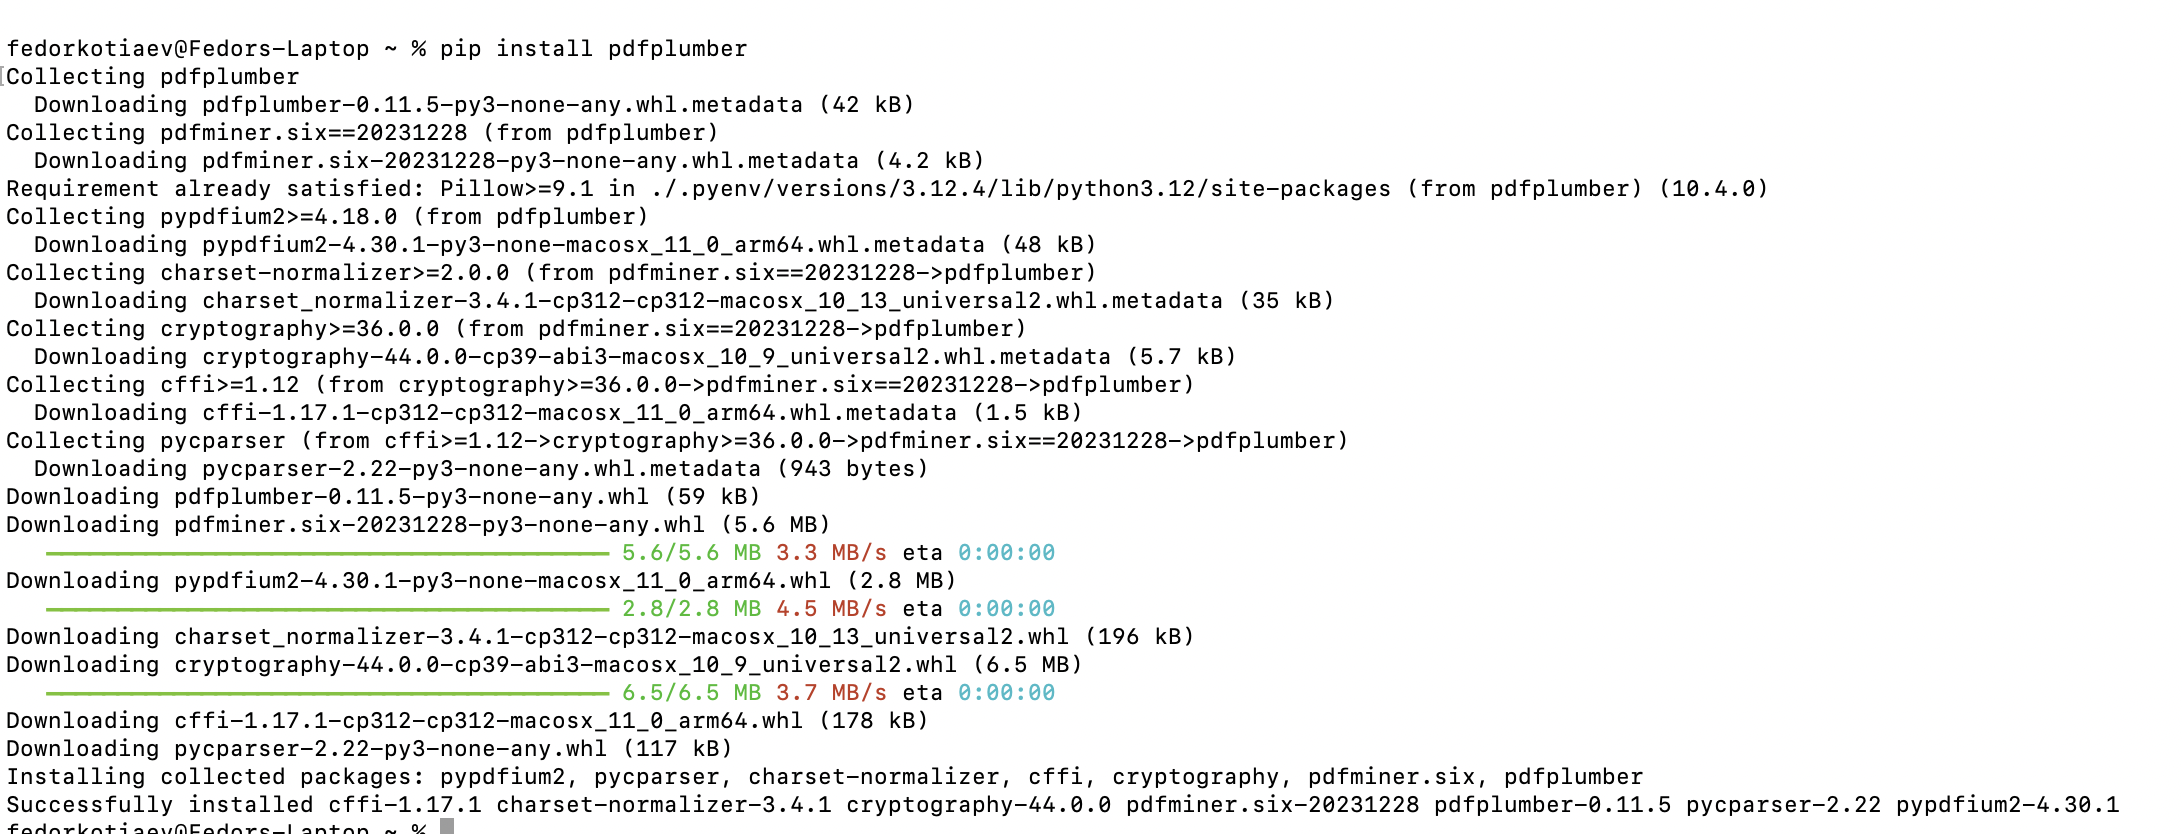
\includegraphics[scale=0.45]{pdfplumber/installationexample.png}
\caption{PDFPlumber Example: Output after installing \texttt{pdfplumber} via pip.}
\label{fig:PDFPlumber install example}
\end{figure}

For more details, visit the official [PyPI Documentation](https://pypi.org/project/pdfplumber/).
\newpage
\section{Working Example PDF}
\label{sec:example pdf}

Throughout this document, we will work with an example PDF file (see Figure~\ref{fig:PDFPlumber example pdf}) that contains four types of objects: text, tables, images, and curves. This file demonstrates how \texttt{pdfplumber} handles diverse PDF elements in practice.\cite{Singer:2022}

\begin{figure}[h!]
\centering
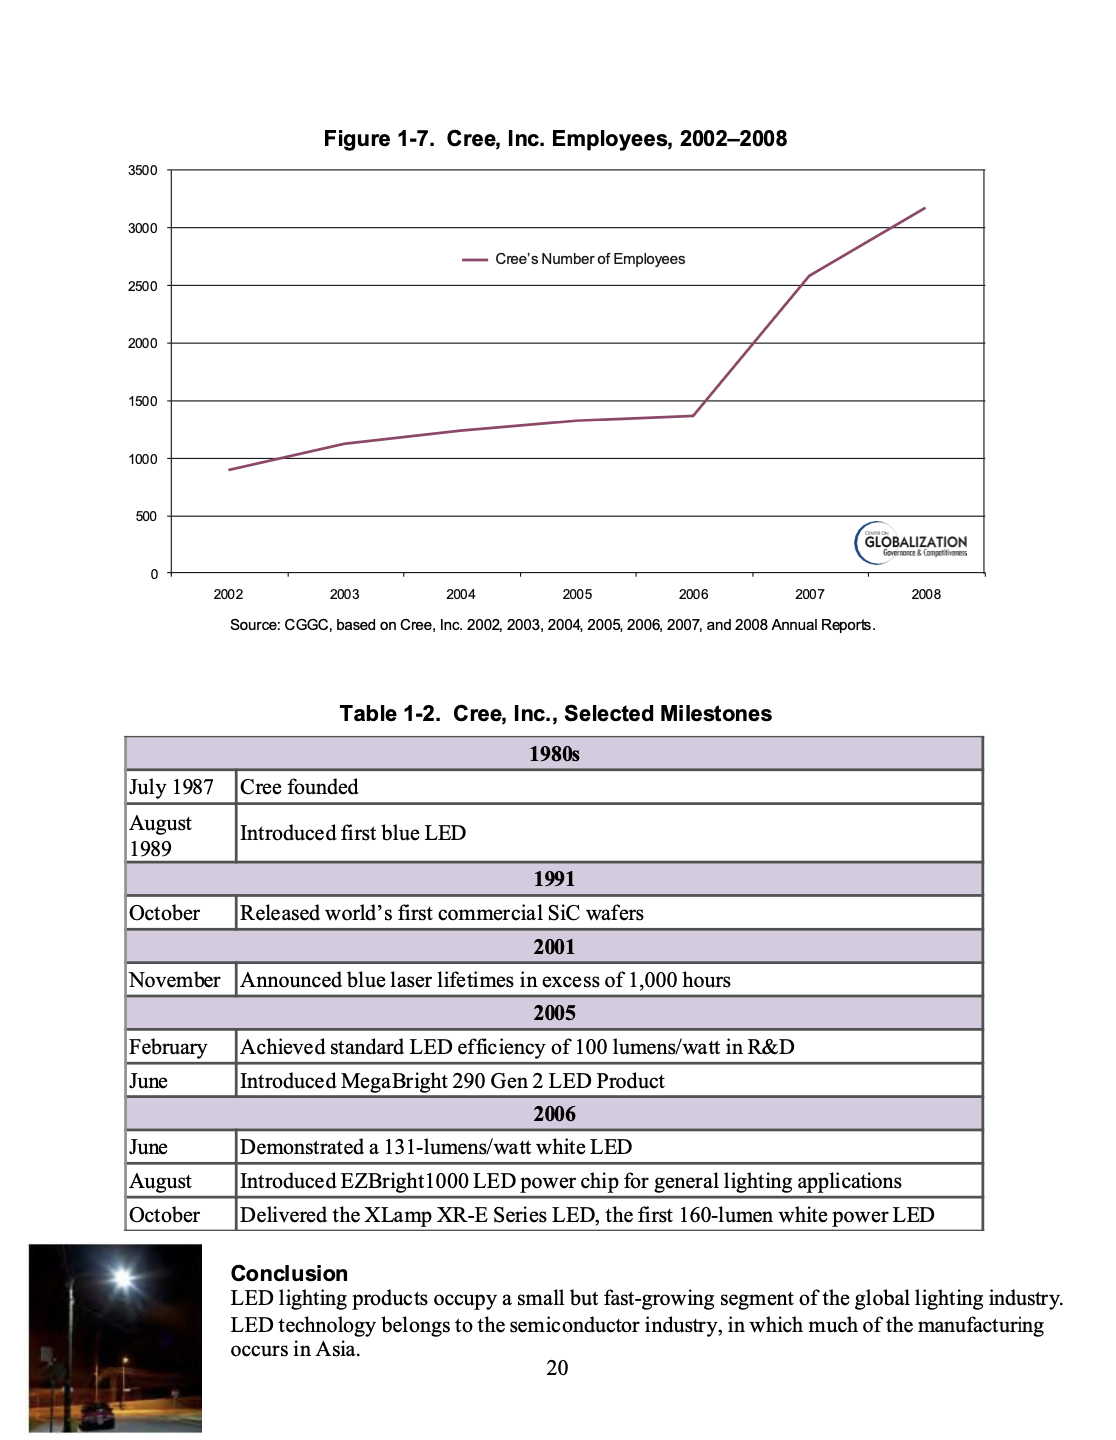
\includegraphics[scale=0.5]{pdfplumber/pdfplumberexample.png}
\caption{PDFPlumber Image of the example PDF file used in this documentation.}
\label{fig:PDFPlumber example pdf}
\end{figure}

\section{Extracting Text}
\label{sec:extracting text}

Text extraction involves retrieving textual content from a PDF in machine-readable form. \texttt{pdfplumber} processes the internal structure of PDFs, extracting text based on character positioning, fonts, and bounding boxes. This method is most effective for structured, non-scanned PDFs.\cite{Singer:2022}

\subsection{Demonstration Example}
Figure~\ref{fig:PDFPlumber text debug} illustrates the extracted text from a PDF page.

\begin{figure}[h!]
\centering
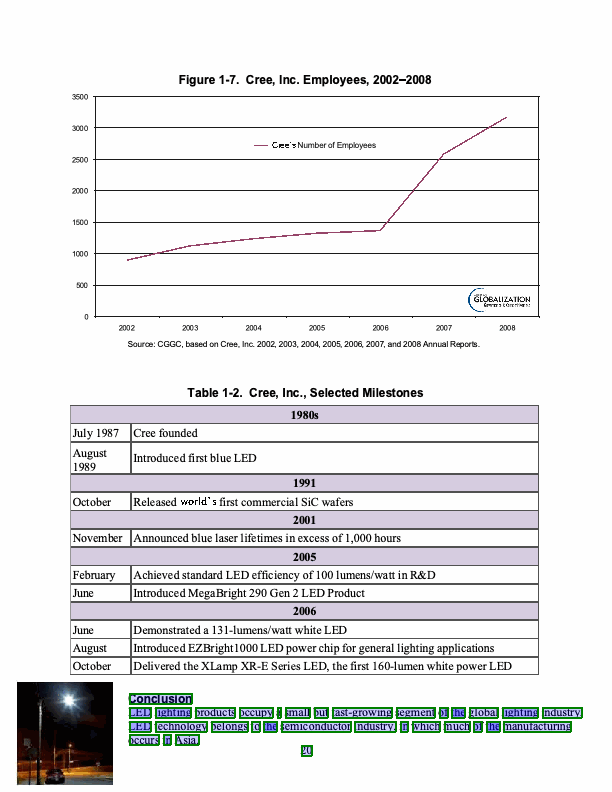
\includegraphics[scale=0.5]{pdfplumber/TextDebug.png}
\caption{PDFPlumber Example: Extracted text from a PDF page.}
\label{fig:PDFPlumber text debug}
\end{figure}

\subsection{Code Example}
\begin{lstlisting}[language=Python, caption={PDFPlumber Extracting text from a PDF.}]
import pdfplumber

with pdfplumber.open("example.pdf") as pdf:
    text = pdf.pages[0].extract_text()
    print(text)
\end{lstlisting}

\subsection{Code Location}
Click [\href{run:../Code/General/pdfplumber/text.py}{PDFPlumber Open Text Extraction Code}] to view the full code.

\section{Extracting Tables}
\label{sec:extracting tables}

Table extraction identifies and retrieves tabular data from PDFs by analyzing the alignment of text and graphical elements like lines. It converts tabular content into structured data, such as a list of lists, making it suitable for further analysis.

\subsection{Demonstration Example}
Figure~\ref{fig:PDFPlumber table debug} demonstrates the detected table from a PDF page.

\begin{figure}[h!]
\centering
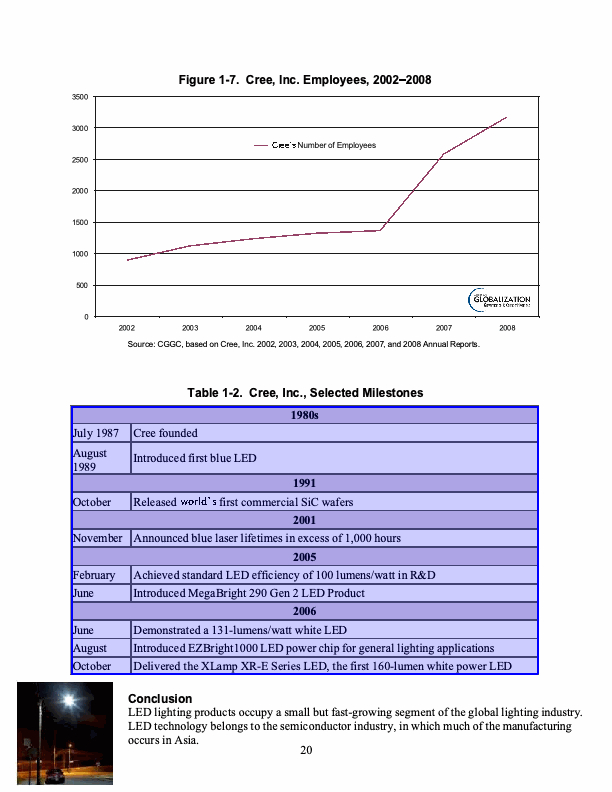
\includegraphics[scale=0.5]{pdfplumber/TableDebug.png}
\caption{PDFPlumber Example: Detected table from a PDF page.}
\label{fig:PDFPlumber table debug}
\end{figure}

\subsection{Code Example}
\begin{lstlisting}[language=Python, caption={PDFPlumber Extracting tables from a PDF.}]
import pdfplumber

with pdfplumber.open("example.pdf") as pdf:
    page = pdf.pages[0]
    table = page.extract_table()
    print(table)
\end{lstlisting}

\subsection{Code Location}
Click [\href{run:../Code/General/pdfplumber/table.py}{PDFPlumber Open Table Extraction Code}] to view the full code.

\section{Extracting Images}
\label{sec:extracting images}

Image extraction retrieves embedded images and their associated metadata, such as dimensions and bounding box coordinates, from a PDF. This feature is essential for handling visual content in documents.\cite{Singer:2022}

\subsection{Demonstration Example}
Figure~\ref{fig:PDFPlumber image debug} shows the extracted images from a PDF page.

\begin{figure}[h!]
\centering
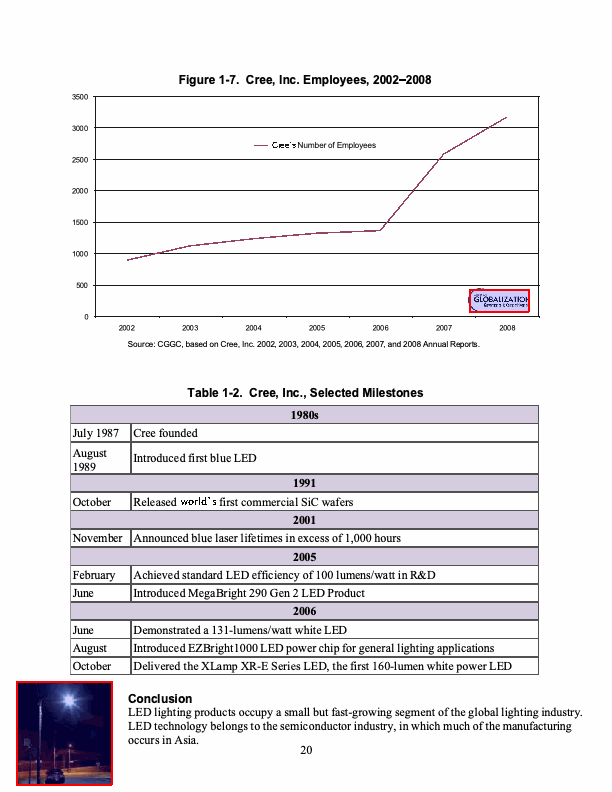
\includegraphics[scale=0.5]{pdfplumber/ImageDebug.png}
\caption{PDFPlumber Example: Extracted images from a PDF page.}
\label{fig:PDFPlumber image debug}
\end{figure}

\subsection{Code Example}
\begin{lstlisting}[language=Python, caption={PDFPlumber Extracting images from a PDF.}]
import pdfplumber

with pdfplumber.open("example.pdf") as pdf:
    page = pdf.pages[0]
    images = page.images
    for img in images:
        print(img)
\end{lstlisting}

\subsection{Code Location}
Click [\href{run:../Code/General/pdfplumber/image.py}{PDFPlumber Open Image Extraction Code}] to view the full code.

\section{Extracting Curves}
\label{sec:extracting curves}

Curve extraction detects and retrieves vector graphics, such as lines and shapes, from a PDF. This method is useful for analyzing graphical elements, such as charts or annotations.\cite{Singer:2022}

\subsection{Demonstration Example}
Figure~\ref{fig:PDFPlumber curve debug} highlights the extracted curves from a PDF page.

\begin{figure}[h!]
\centering
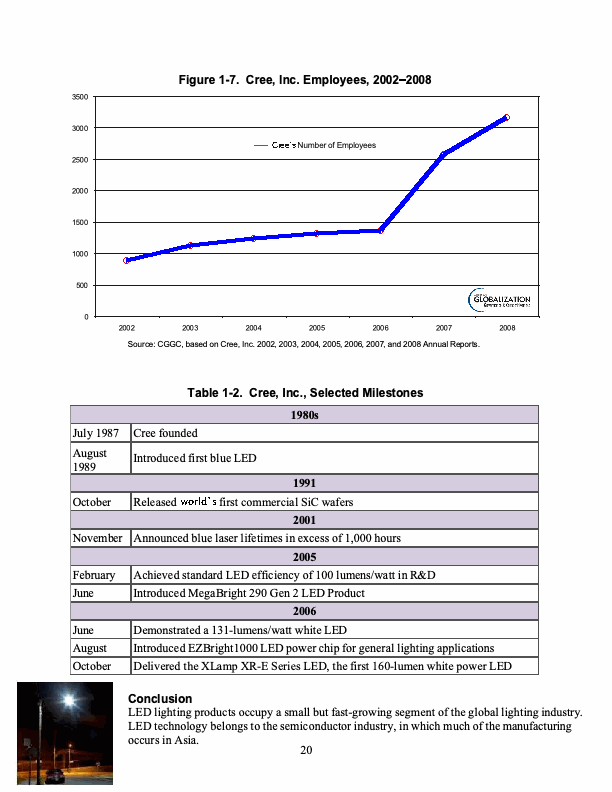
\includegraphics[scale=0.5]{pdfplumber/CurveDebug.png}
\caption{PDFPlumber Example: Extracted curves from a PDF page.}
\label{fig:PDFPlumber curve debug}
\end{figure}

\subsection{Code Example}
\begin{lstlisting}[language=Python, caption={PDFPlumber Extracting curves from a PDF.}]
import pdfplumber

with pdfplumber.open("example.pdf") as pdf:
    page = pdf.pages[0]
    curves = page.curves
    for curve in curves:
        print(curve)
\end{lstlisting}

\subsection{Code Location}
Click [\href{run:../Code/General/pdfplumber/curve.py}{PDFPlumber Open Curve Extraction Code}] to view the full code.

\section{Why Choose \texttt{pdfplumber}?}
\label{sec:whychoose}

\begin{itemize}
    \item Provides detailed object-level access for text, tables, and visual elements.
    \item Includes integrated visual debugging tools for easy analysis.
    \item Supports a wide range of PDFs with precision.\cite{Singer:2022}
\end{itemize}

\section{Further Reading}
\label{sec:furtherreading}

\begin{itemize}
    \item GitHub Repository: \href{https://github.com/jsvine/pdfplumber}{GitHub Repository}
    \item PyPI Documentation: \href{https://pypi.org/project/pdfplumber/}{PyPI Documentation}
\end{itemize}

